\section{Методы редукции размерности}
В этом разделе рассмотрим более подробно упомянутый ранее метод редукции размерности
с помощью кривых Пеано, заполняющих пространство, и сравним между собой разные модификации различных кривых.
Кроме прямой редукции размерности с помощью кривых типа Пеано, существует и способ, сводящий одну задачу оптимизации к
множеству вложенных задач оптимизации: многошаговая схема \cite{strongin1978}:
\begin{equation}
  \label{eq:3}
  \min_{y \in D} \varphi(y) = \min_{y_1 \in [a_1, b_1]} \dots \min_{y_N \in [a_N, b_N]} \varphi(y_1, \dots, y_N).
\end{equation}

В рамках многошаговой схемы каждое вычисление целевой функции по переменной \(y_1\) во внешней задаче оптимизации влечёт за собой
проведение ещё \(N-1\) вложенной оптимизации. Недостатками данной схемы является её низкая экономичность в плане количества
обращений к целевой функции и отсутствие теоретической гарантии сходимости IAGS при наличии функциональных ограничений
(в некоторых случаях целевые функции во вложенных задачах перестают удовлетворять условию Липшица). В качестве обобщения
многошаговой схемы было предложено вложенную оптимизацию вести не по одиночным переменным, а по блокам переменных \cite{globalizerSystem}.
К многомерным вложенным задачам в таком случае можно применить редукцию размерности с помощью кривых типа Пеано,
поэтому выявление наиболее эффективного типа кривой имеет смысл и для ускорения сходимости в случае блочной многошаговой схемы.

\subsection{Инъективная развёртка}

Для редукции размерности задач оптимизации в рамках информационно-статистического подхода
применяются кривые типа Пеано, заполняющие пространство (развёртки) \cite{Sergeyev2013, strongin1978,
Gergel2009, Strongin2000}. Такие кривые отображают отрезок \([0,1]\) на \(N\)-мерный гиперкуб \(D\).

После редукции размерности исходная многомерная задача (\ref{eq:task}) преобразуется в одномерную задачу
следующего вида:
\begin{equation}
\label{eq:oneDimTask}
\varphi(y(x^*))=\min\{\varphi(y(x)):x\in [0,1]\}.
\end{equation}

Стоит отметить, что подстановка развёртки в Липшицеву функцию  % minimized
из (\ref{eq:task}) порождает одномерную функцию \(\varphi(y(x))\), которая удовлетворяет условию Гёльдера:
\begin{equation}
\label{eq:holder}
|\varphi(y(x_1))-\varphi(y(x_2))|\leq H{|x_1-x_2|}^{\frac{1}{N}}, x_1,x_2\in[0,1],
\end{equation}
где константа $H$ удовлетворяет неравенству \(H\leqslant2L\sqrt{N+3}\), \(L\) -- константа Липшица из (\ref{eq:lip}),
и \(N\) -- размерность задачи (\ref{eq:task}).

На Pис. \ref{fig:evolvent_example} приведена одномерная функция, полученная после применения развёртки к
парабалоиду вращения \(\varphi(y)=y_1^2+y_2^2\). Точка с координатами \((0;0)\) имеет несколько одномерных прообразов
и глобальный минимум целевой функции в ней расщепился на три глобальных минимума одномерной функции, полученной в результате
редукции. Этот пример демонстрирует последствия потери информации об окрестности точки \((0;0)\) при редукции размерности.

\begin{figure}[ht]
    \center
    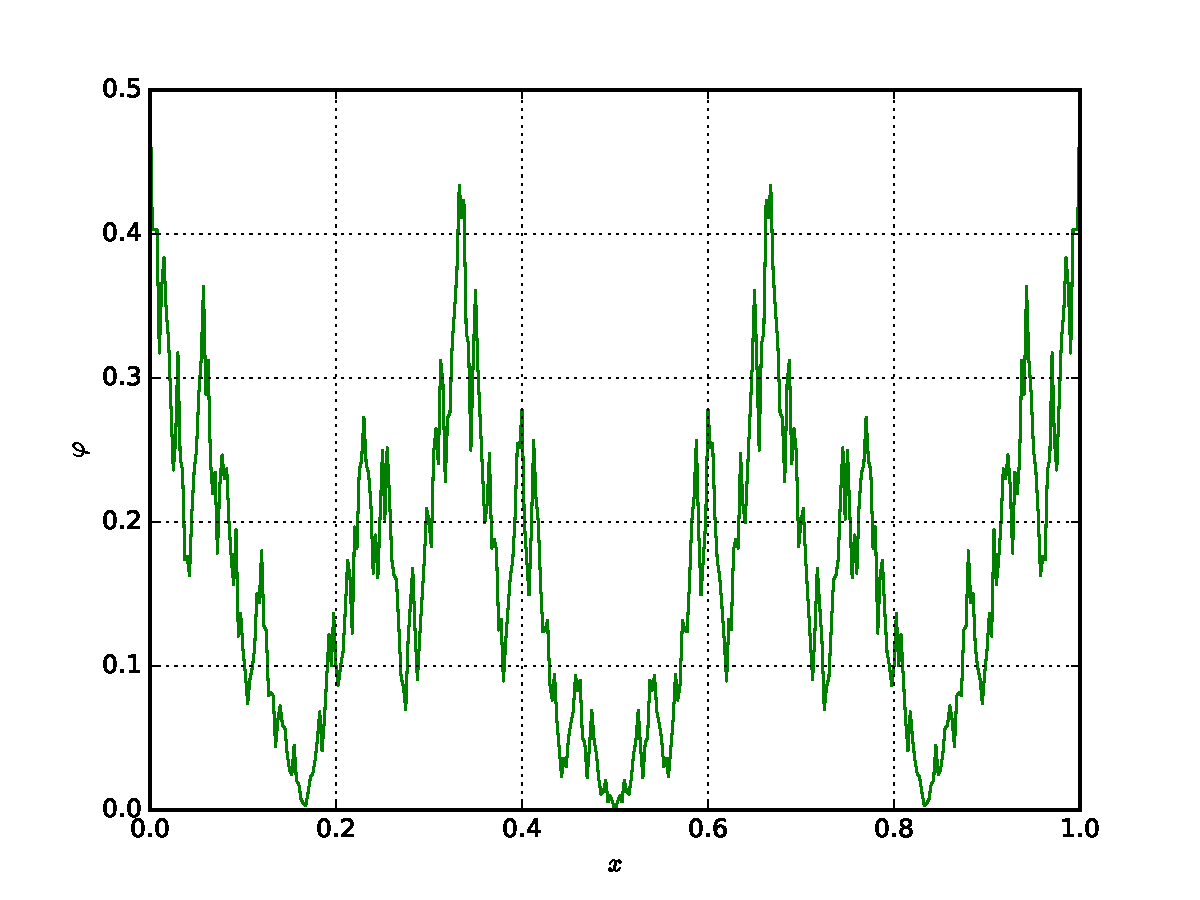
\includegraphics[width=0.75\textwidth]{images/map_paraboloid.pdf}
    \caption{Пример одномерной функции, порождённой развёрткой}
    \label{fig:evolvent_example}
\end{figure}

Алгоритмы численного построения аппроксимаций кривой Пеано приведены в \cite{Strongin2000}.

Вычислительная схема алгоритма, применяющего кривые Пеано для редукции размерности, выглядит следующим образом:
\begin{itemize}
  \item Алгоритм оптимизации выполняет минимизацию редуцированной одномерной функции
  \(\varphi(y(x))\) из (\ref{eq:oneDimTask}),
  \item После нахождения точки следующего испытания \(x\), её многомерный образ \(y\)
  вычисляется с использованием развёртки \(y(x)\),
  \item Значение исходной многомерной функции \(\varphi(y)\) вычисляется в точке \(y\in D\),
  \item Вычисленное значение \(z=\varphi(y)\) используется как значение одномерной редуцированной функции \(\varphi(y(x))\) в точке \(x\).
\end{itemize}

%------------------------------------------------------------------------------
\subsection{Сдвиговые развёртки}
\label{sec:shifted}

Применение кривой типа Пеано для редукции размерности приводит к потере локальной информации об окрестности многомерных точек
в пространстве $\mathbb{R}^N$ (см. \cite{Strongin1992}).
Одним из способов частично решить эту проблему является использование множества развёрток \cite{Strongin1992}:
\begin{equation}%\label{eq:142}
Y_L(x)=\left\{y^0(x),\ y^1(x),...,\ y^L(x)\right\}
\end{equation}
вместо одной кривой Пеано $y(x)$ (см. \cite{Strongin1992,Strongin2000, Strongin1991}).

Такой набор отображений может быть получен путём сдвига исходной развёртки $y^0(x)$ на $2^{-l},0
\leq l \leq L$ по каждой из координат. Каждая из развёрток определена на своём гиперкубе $D_l=
\left\{y \in R^N: -2^{-1} \leq y_i+2^{-l} \leq 3 \cdot 2^{-1},\ 1\leq i\leq N\right\},\ 0 \leq l \leq
L$.

На Рис.~\ref{fig:shifted_ev} пунктирной линией обозначен образ интервала $[0,1]$, полученный с помощью $y^0(x),\
x\in [0,1],$. Поскольку гиперкуб $D$ из (\ref{eq:task}) принадлежит пересечению
семейства гиперкубов $D_l$, необходимо ввести дополнительное ограничение:
\begin{equation}\label{6_g0}
g_0(y)=\max\left\{\left|y_i\right| - 2^{-1}:\ 1\leq i\leq N\right\},
\end{equation}
тогда гиперкуб $D$ можно представить в виде
\[
D=\left\{y^l(x):\; x\in [0,1],\ g_0(y^l(x))\leq 0 \right\},\ 0\leq l \leq L,
\]
т.е. $g_0(y) \leq 0$ если $y\in D$, иначе $g_0(y)>0$. Следовательно, любая точка $y \in D$
имеет прообраз $x^l \in [0,1]$, определяемый соответствующей развёрткой $y^l(x),\ 0\leq l\leq L$.

Таким образом, каждая развёртка $y^l(x),\ 0\leq l \leq L,$ порождает свою собственную задачу вида
(\ref{eq:task}), имеющую расширенную (по сравнению с $D$) область поиска $D_l$
и дополнительное ограничение-неравенство с левой частью вида (\ref{6_g0})
\begin{equation}\label{6_problem_l}
\min{\left\{\varphi(y^l(x)):x\in [0,1], \; g_j(y^l(x))\leq 0, \; 0 \leq j \leq m\right\}}, \ 0 \leq l \leq L.
\end{equation}
При этом, $L$ копий метода AGS решают каждую из указанных задач, на каждой итерации обмениваясь многомерными точками
следующего испытания и добавляя их прообразы в свою поисковую информацию. Такая схема имеет смысл только при
наличии $L$ параллельных вычислительных ядер или процессоров.

\begin{figure}[ht]
    \centering
    \subfloat[Две сдвиговые развёртки, определённые на гиперкубах $D_0$ и $D_1$]{{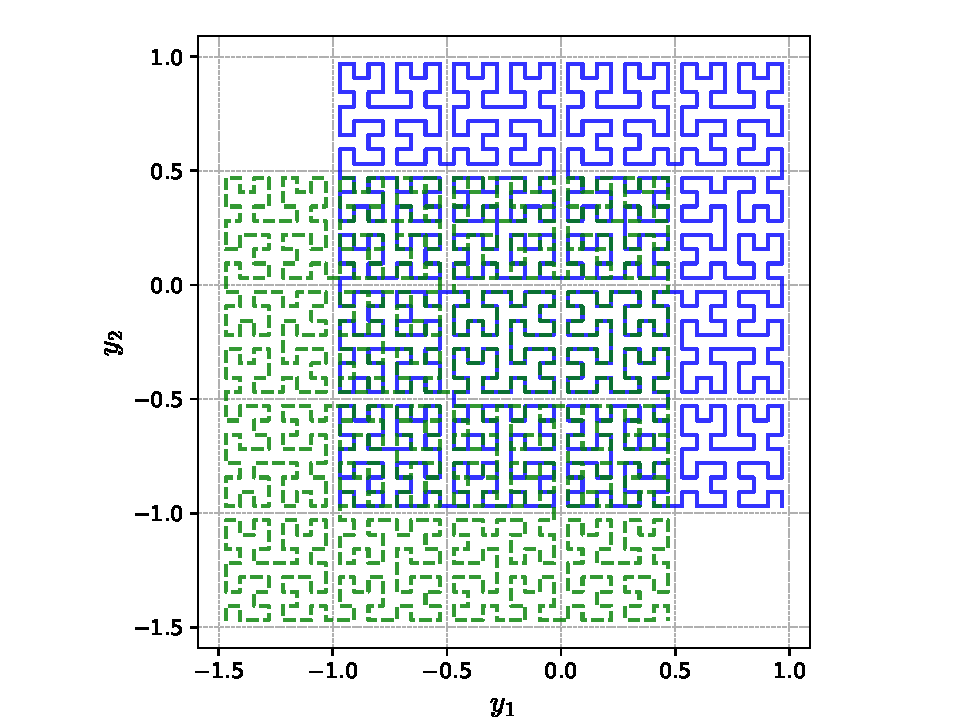
\includegraphics[width=.5\textwidth]{evolvents/shifted.pdf}}\label{fig:shifted_ev}}
    %\subfloat[Hypercubes $D_l$]{{\includegraphics[width=.4\textwidth]{pictures/shifted_cube.png}}\label{fig:shifted_cube}}
    \subfloat[Две вращаемые развёртки на одной плоскости]{{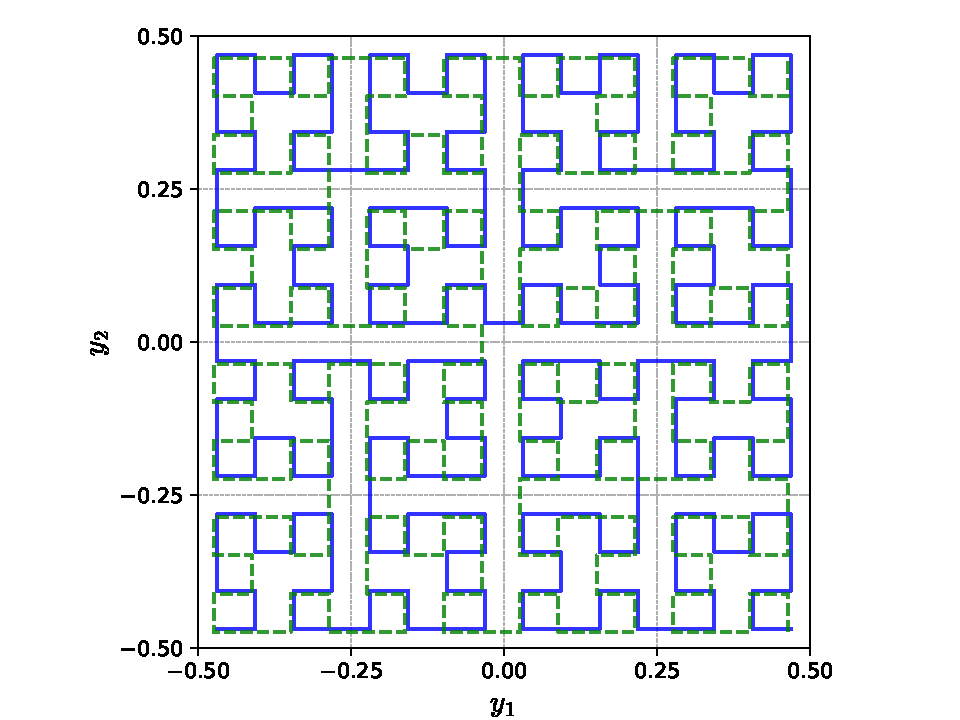
\includegraphics[width=.5\textwidth]{evolvents/rotated.pdf}}\label{6_fig_9}}
    \caption{Различные развёртки, построенные с низкой плотностью}
\end{figure}

%------------------------------------------------------------------------------
\subsection{Вращаемые развёртки}
Схема построения множества развёрток (здесь и далее будем называть, развёртки, порождённые ей сдвиговыми
или $S$-развёртками), описанная в Секции~\ref{sec:shifted}, позволяет сохранять часть информации
о близости точке в многомерном пространстве и, таким образом, обеспечивает более точную (по сравнению с одной развёрткой)
оценку константы Гёльдера в процессе оптимизации. Однако, однако, этот подход имеет недостаток в виде наличия дополнительного ограничения
что затрудняет построение эффективных реализаций алгоритма оптимизации на базе $S$-развёрток (см. конец Секции~\ref{sec:seq_comp}).

Чтобы обойти сложности, возникающие при работе с $S$-развёртками и одновременно сохранить часть информации об окрестностях точек
$N$-мерном вещественном пространстве, была редложена ещё одна схема построения множества развёрток.
Эта схема предполагает вместо получения группы развёрток делать сдвиг не сдвиг кривой Пеано по диагонали гиперкуба, а
её вращение относительно центра координат \cite{Gergel2009}.
На Рис.~\ref{6_fig_9} представлены две развёртки, аппроксимирующие кривую Пеано при $N=2$.
Получая новые развёртки путём отражения относительно осей координат, можно породить множество развёрток
мощностью до $2^N$. При этом дополнительное ограничение $g_0(y)$ из (\ref{6_g0}), необходимое для получения
набора $S$-развёрток, отсутствует.
%Минусом вращаемых развёрток, по сравнению со сдвиговыми, является отсутствие теоретической гарантии
%получения близких прообразов для близких многомерных точек.
%Taking into account the initial mapping, one can conclude that current implementation of the

%------------------------------------------------------------------------------
\subsection{Неинъективная развёртка}

Как уже было сказано в секции \ref{sec:shifted}, потеря информации о близости точек в многомерном
пространстве может быть частично скомпенсирована использованием множественных отображений $Y_L(x)=\{y^1(x),...,y^L(x)\}$.
Однако, сама по себе кривая типа Пеано сохраняет в себе часть этой информации: она не является инъективым отображением,
поэтому имея один образ $y(x)\in \mathbb{R}^N$, можно получить несколько несколько отличных $x$ прообразов $t_j\in[0,1], t_j \not = x$,
которые затем могут быть добавлены в поисковую информацию индексного метода.

Кривая типа Пеано, используемая в (\ref{eq:oneDimTask}) для редукции размерности, определяется через предельный переход,
поэтому не может быть вычислена непосредтвенно. При численной оптимизации используется некоторое её приближение, являющееся
инъективной кусочно-линейной кривой. В \cite{strongin1978} было предложено неинъективное отображение равномерной сетки на
отрезка $[0,1]$ на равномерную сетку в гиперкубе $D$. Каждый многомерный узел может иметь до $2^N$ одномерных прообразов.
На рис. \ref{fig:noninjective} крестиками обозначена сетка в пространстве $\mathbb{R}^2$, для двух узлов которой
указаны соответствующие им одномерное прообразы из $[0,1]$ (отмечены квадратами и кругами). Каждый указанный узел имеет по 3 прообраза.

Недостатком неинъективной развёртки является потенциально большое количество прообразов (до $2^N$).
% и невозможность использования параллельной схемы для множественных отображений из секции \ref{sec:parallel_evolvents}.


%------------------------------------------------------------------------------
\subsection{Гладкая развёртка}

Рассмотренные в предыдущих пунктах способы построения развертки строят кривую $y(x)$, которая не является
гладкой (см. рис. \ref{fig:shifted_ev}). Отсутствие гладкости может негативно сказаться на свойствах редуцированной
одномерной функции $\varphi(y(x))$, т.к. гладкая кривая более качественно передает информации о возрастании/убывании
исходной функции. На основе исходного алгоритма построения негладкой развертки было предложен обобщенный алгоритм
\cite{Goryachih2017}, позволяющий строить гладкую развёртку. Для иллюстрации на рис. \ref{fig:smooth} изображена гладкая
развертка в двумерном случае. Недостатком гладкой развёртки является в несколько раз большая сложность вычисления по
сравнению с кусочно-линейными кривыми (требуется вычислять нелинейные гладкие функции). Причём с ростом точности аппроксимации и
размерности количество интервалов гладкости увеличивается и сложность вычисления кривой нарастает.

\begin{figure}[ht]
    \centering
    \subfloat[Гладкая развёртка]{{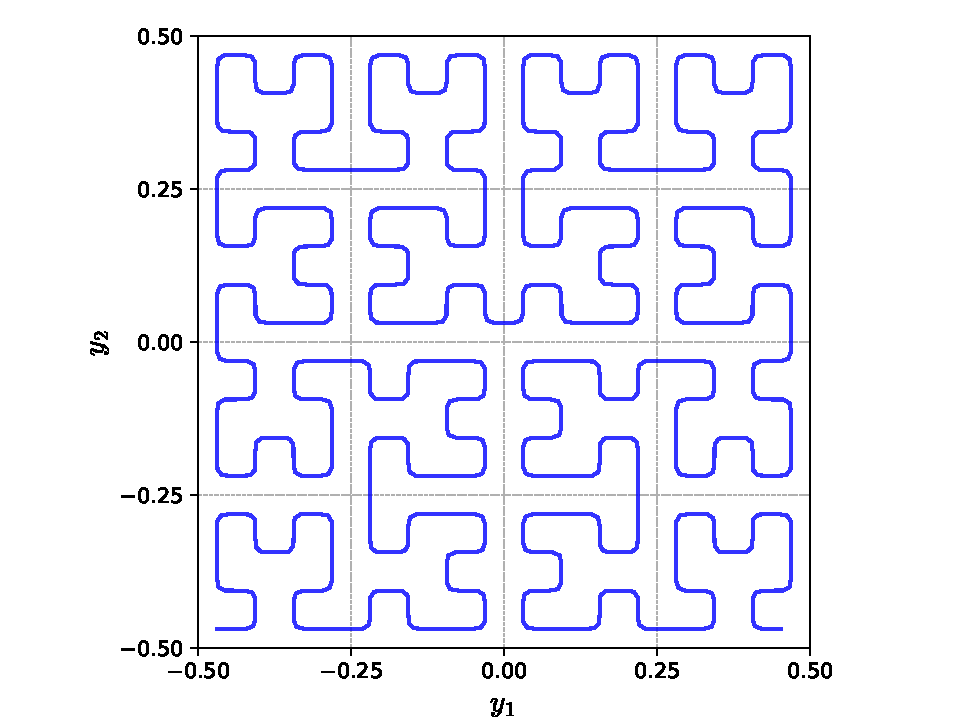
\includegraphics[width=.6\textwidth]{evolvents/smooth.pdf}}\label{fig:smooth}}
    \subfloat[Неинъективная развёртка]{{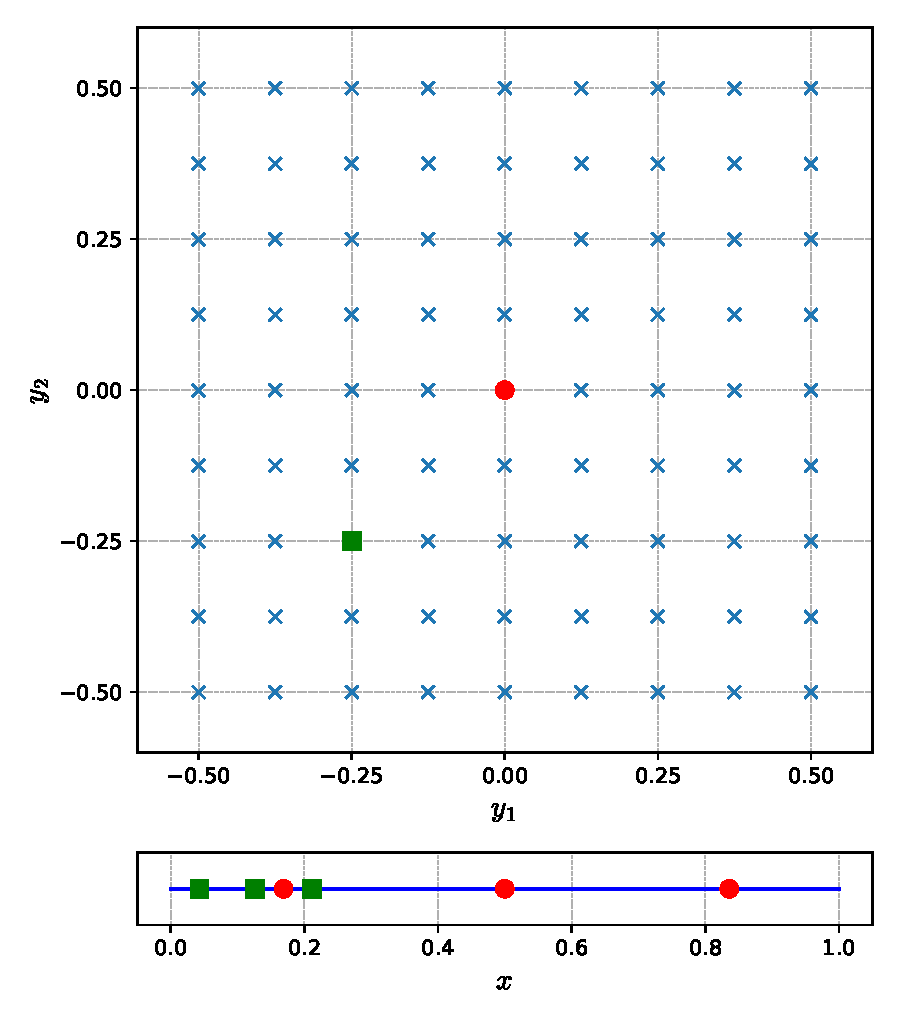
\includegraphics[width=.4\textwidth]{evolvents/noninjective.pdf}}\label{fig:noninjective}}
    \caption{Различные развёртки, построенные с низкой плотностью}
\end{figure}

\subsection{Сравнение развёрток}
\label{sec:seq_comp}
Сравнение скорости сходимости IAGS с различными типами развёткок проводилось в соответствии с методикой, описанной в
Секции \ref{sec:comp_tools}. С целью понять, обладает ли какой-либо из перечисленных ранее типов развёрток существенным преимуществом над другими,
были построены операционные характеристики индексного метода с различными типами развёрток на наборах задач GKLS 2d Simple и GKLS 3d Simple.

Во всех экспериментах параметр плотности построения развёрток $m=12$. Минимальное значение параметра надёжности \(r\) было найдено
для каждого типа развёртки перебором по равномерной сетке с шагом \(0.1\).

На классе GKLS 2d Simple при минимальном \(r\) неинъективная и гладкая развёртка обеспечивают более быструю сходимость
(рис. \ref{fig:gkls2d_opt}). То же самое, наблюдается и при \(r=5.0\) (рис. \ref{fig:gkls2d_acc}). В последнем случае сдвиговая и
вращаемая развёртки начинают отставать от остальных, т.к. значение \(r=5.0\) является завышенным для них.
\begin{figure}[ht]
    \centering
    \subfloat[$r=5.0$]{{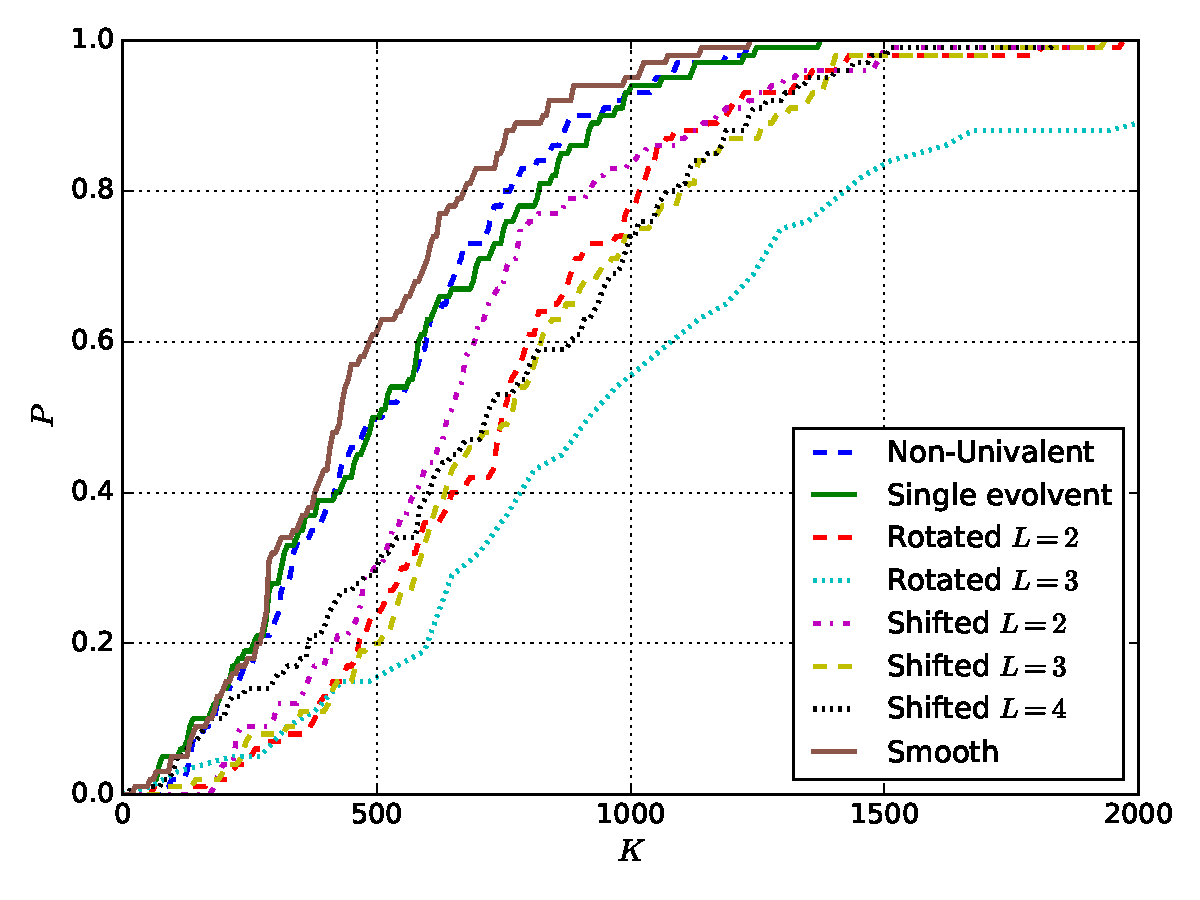
\includegraphics[width=.5\textwidth]{evolvents/gklsS2d_same_r_opt_pt_op.pdf}}\label{fig:gkls2d_acc}}
    \subfloat[Minimal $r$]{{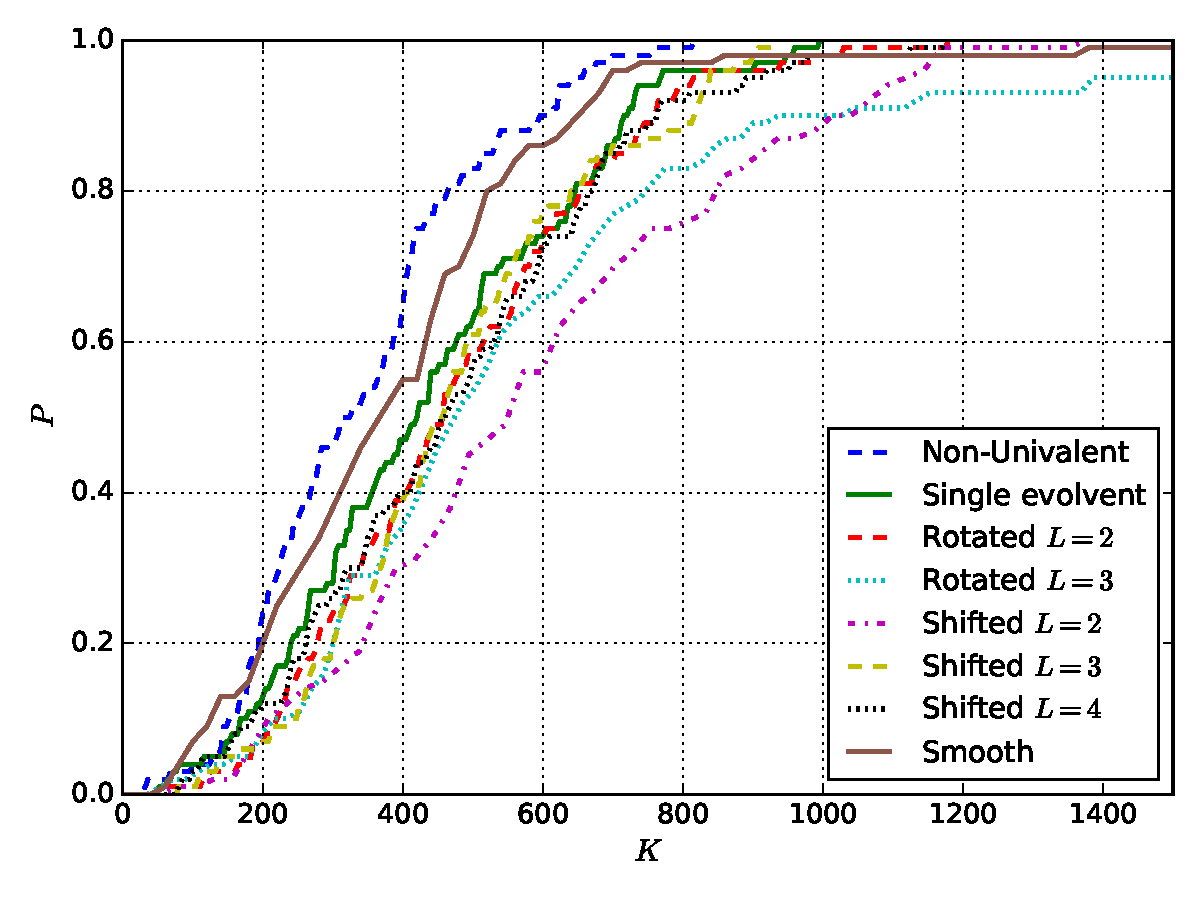
\includegraphics[width=.5\textwidth]{evolvents/gklsS2d_opt_pt_op.pdf}}\label{fig:gkls2d_opt}}
    \caption{Операционные характеристики на классе GKLS 2d Simple}
\end{figure}

На классе GKLS 2d Simple при минимальном \(r\) неинъективная и множественные развёртки имеют значительное
преимущество над единственной развёрткой (рис. \ref{fig:gkls3d_opt}). Значение \(r=4.5\) является завышенным для
вращаемой и сдвиговой развёрток (рис. \ref{fig:gkls3d_acc}).

\begin{figure}[ht]
    \centering
    \subfloat[$r=4.5$]{{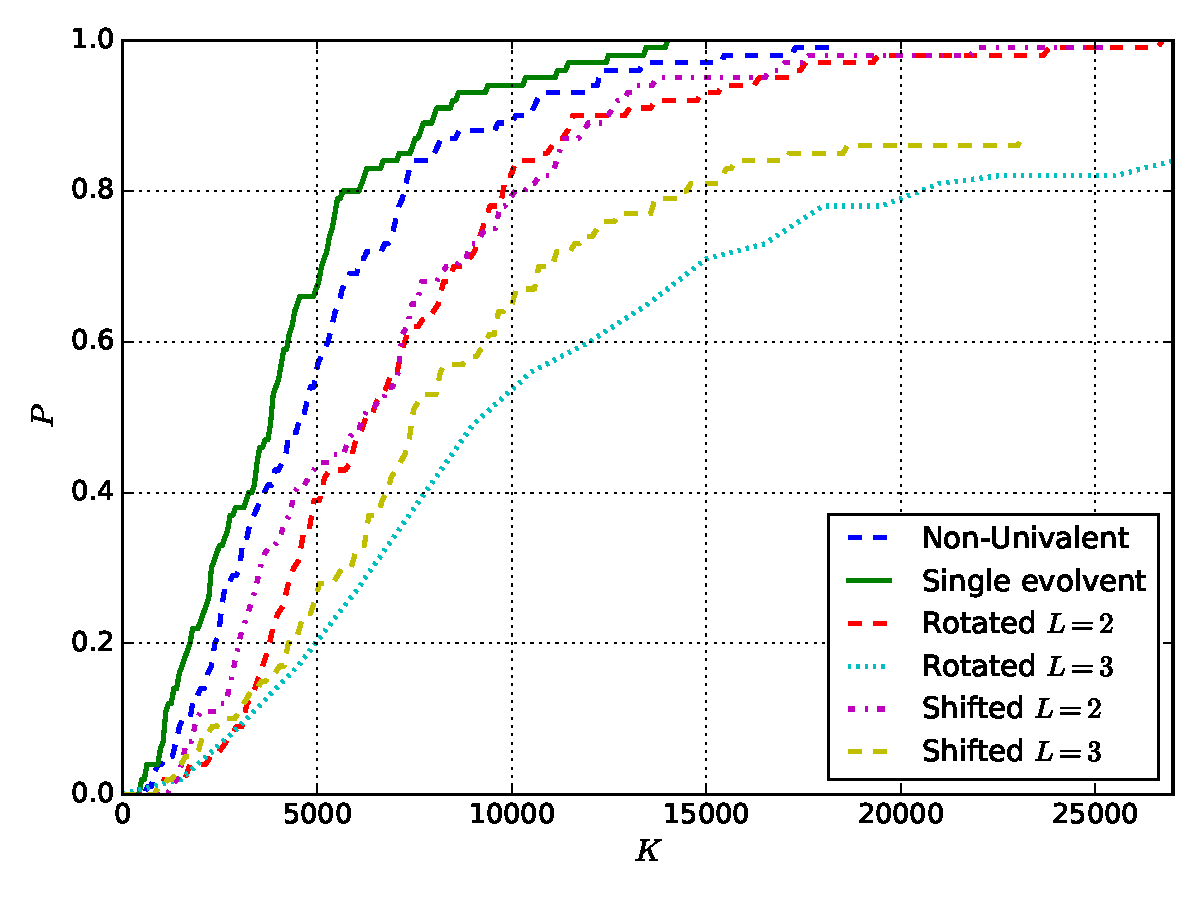
\includegraphics[width=.5\textwidth]{evolvents/gklsS3d_same_r_opt_pt_op.pdf}}\label{fig:gkls3d_acc}}
    \subfloat[Minimal $r$]{{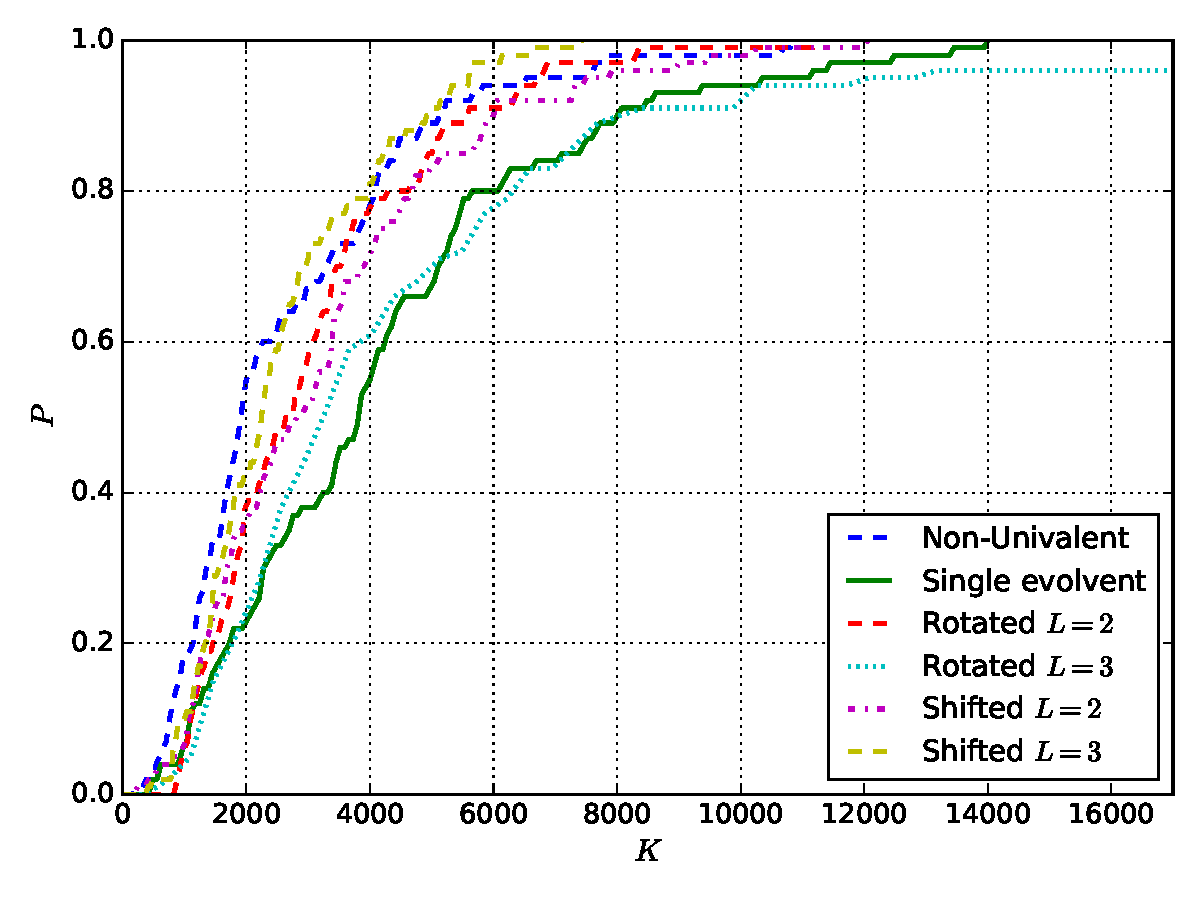
\includegraphics[width=.5\textwidth]{evolvents/gklsS3d_opt_pt_op.pdf}}\label{fig:gkls3d_opt}}
    \caption{Операционные характеристики на классе GKLS 3d Simple class}
\end{figure}

\paragraph{Накладные расходы при использовании сдвиговой развёртки.}
Во всех представленных выше экспериментах при построении операционной характеристики учитывалось количество
вычислений целевой функции из класса GKLS, однако в случае сдвиговой развёртки индексный метод решает задачу
с ограничением \(g_0\) из (\ref{6_g0}). В точках, где \(g_0\) нарушено, значение целевой функции не вычисляется.
Эти точки, тем не менее, хранятся в поисковой информации, создавая дополнительные расходы вычислительных ресурсов.
В таблице \ref{tab:shifted_g0} приведено среднее количество обращение к \(g_0\) и целевой функции. При \(L=3\)
ограничение \(g_0\) вычисляется почти в 20 раз чаще, чем целевая функция \(\varphi\), т. е. \(95\%\)
всей поисковой информации приходится на вспомогательные точки. Такие накладные расходы приемлемы при решении
задач малой размерности с трудоёмкими целевыми функциями, но при росте размерности и общего количества испытаний выгоднее
использовать другие типы развёрток.

\begin{table}
\begin{center}
\caption{Среднее количество вычислений \(g_0\) и \(\varphi\) при решении задач класса GKLS 3d Simple с помощью сдвиговой развёртки}
  \begin{tabular}{|l|{c}|{c}|{c}|}
    \hline
  $L$ & $calc(g_0)$ & $calc(\varphi)$ & $\frac{calc(g_0)}{calc(\varphi)}$ ratio \\
  \hline
  2 & 96247.9  & 6840.14 & 14.07\\
  \hline
  3 & 153131.0 & 7702.82 & 19.88\\
  \hline
  \end{tabular}
  \label{tab:shifted_g0}
\end{center}
\end{table}

\subsection{Итоги сравнения}

В результате проведённого сравнения различных способов редукции размерности, основанных на отображениях типа кривой Пеано,
можно сделать вывод о том, что для построения базовой версии AGS с практической стороны
выгоднее использовать единственную кривую Пеано, кроме случаев низкой размерности или чрезвычайно трудоёмкого вычисления целевой
функции. Из множественных отображений оптимальным выбором будет использование вращаемых развёрток. Поскольку результаты, полученные для
алгоритма с одной развёрткой непосредственно распространяются на алгоритмы с вращаемыми развёртками, далее будем рассматривать
только случай единственной кривой Пеано.
